\documentclass[border=4pt, multi, tikz]{standalone}
\usepackage{import}
\subimport{./PlotNeuralNet/layers/}{init}
\usepackage{mathptmx}
\usepackage{amsmath,amssymb}
\usepackage{graphicx}
\usetikzlibrary{positioning,3d,arrows.meta,calc,fit,backgrounds,shapes.geometric,decorations.pathreplacing}

\definecolor{cIn}      {HTML}{C3CEDC}   % raw points / pillar builder
\definecolor{cLinear}  {HTML}{6E97C7}   % Linear + BN + ReLU
\definecolor{cAttn}    {HTML}{B47CC7}   % grouped vector attention
\definecolor{cPool}    {HTML}{E07B7B}   % masked max-pool
\definecolor{cCanvas}  {HTML}{74B58C}   % BEV canvas
\definecolor{cPrior}   {HTML}{E9C46A}   % learned positional prior
\definecolor{cS0}      {HTML}{93C47D}   % backbone stage 0  (k=13)
\definecolor{cS1}      {HTML}{E8D07A}   % backbone stage 1  (k=11)
\definecolor{cS2}      {HTML}{E2A85F}   % backbone stage 2  (k=9)
\definecolor{cNgfm}    {HTML}{4FA8AC}   % normal-guided modulation
\definecolor{cUp1}     {HTML}{A8D5BA}   % upsample stage 1
\definecolor{cUp2}     {HTML}{7FC4A0}   % upsample stage 2
\definecolor{cHead}    {HTML}{3A5F8F}   % CenterHead
\definecolor{cLoss}    {HTML}{E63946}   % NGFM auxiliary loss
\definecolor{cInk}     {HTML}{1A1A1A}
\definecolor{cMuted}   {HTML}{55606B}
\definecolor{cGrid}    {HTML}{93A0AD}
\definecolor{cAux}     {HTML}{8A6FB0}   % training-only signals

\begin{document}
\begin{tikzpicture}[
    font=\fontsize{17}{19}\selectfont,
    lbl/.style   ={text=cInk, align=center, inner sep=0.8pt},
    mod/.style   ={lbl, font=\fontsize{19.5}{21.5}\selectfont},
    dim/.style   ={lbl, text=cMuted, font=\fontsize{16}{18}\selectfont},
    tag/.style   ={lbl, text=cMuted, font=\fontsize{17}{19}\selectfont},
    flow/.style  ={-{Stealth[length=5.5pt,width=4pt]}, draw=cInk, line width=1pt},
    aux/.style   ={-{Stealth[length=5.5pt,width=4pt]}, draw=cAux, line width=0.9pt,
                   dash pattern=on 3.5pt off 2.5pt},
    leader/.style={draw=cGrid, line width=0.45pt},
    brace/.style ={decorate, decoration={brace, amplitude=4pt}, draw=cMuted, line width=0.5pt},
  ]
% ====== input sweep ======
\node[anchor=west, inner sep=0] (scan) at (0.240,0,0)
    {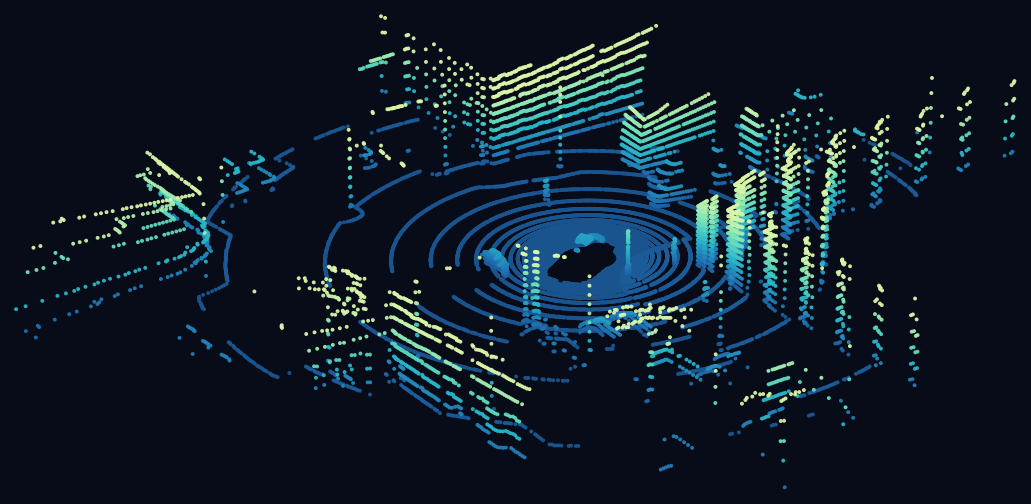
\includegraphics[height=2.30cm]{panels/lidar_scan.png}};
\node[mod, anchor=north, xshift=0.00cm, yshift=-0.10cm] at (2.592,-1.980,0) {\textbf{LiDAR}\\\textbf{sweep}};
% ====== pillar feature builder ======
\pic[shift={(0,0,0)}] at (6.435,0.000,0.000)
    {PlainBox={name=builder, caption=, fill=cIn, opacity=0.95,
        width=0.380, height=2.400, depth=2.400, scale=1}};
\draw[flow] (scan.east) -- (builder-west);
\draw[leader] (6.625,-1.780,0) -- (6.625,-1.920,0);
\node[mod, anchor=north, xshift=0.00cm, yshift=-0.10cm] at (6.625,-1.980,0) {\textbf{Pillar}\\\textbf{features}};
\node[tag, anchor=south, xshift=0.00cm, yshift=-0.10cm] at (6.625,2.450,0) {0.4\,m, $\le8$ pts};
% -- isometric pillar grid `gA` --
\draw[cGrid, opacity=0.85, line width=0.3pt] (8.305,0,-1.080) -- (8.305,0,1.080);
\draw[cGrid, opacity=0.85, line width=0.3pt] (8.665,0,-1.080) -- (8.665,0,1.080);
\draw[cGrid, opacity=0.85, line width=0.3pt] (9.025,0,-1.080) -- (9.025,0,1.080);
\draw[cGrid, opacity=0.85, line width=0.3pt] (9.385,0,-1.080) -- (9.385,0,1.080);
\draw[cGrid, opacity=0.85, line width=0.3pt] (9.745,0,-1.080) -- (9.745,0,1.080);
\draw[cGrid, opacity=0.85, line width=0.3pt] (10.105,0,-1.080) -- (10.105,0,1.080);
\draw[cGrid, opacity=0.85, line width=0.3pt] (10.465,0,-1.080) -- (10.465,0,1.080);
\draw[cGrid, opacity=0.85, line width=0.3pt] (10.825,0,-1.080) -- (10.825,0,1.080);
\draw[cGrid, opacity=0.85, line width=0.3pt] (11.185,0,-1.080) -- (11.185,0,1.080);
\draw[cGrid, opacity=0.85, line width=0.3pt] (11.545,0,-1.080) -- (11.545,0,1.080);
\draw[cGrid, opacity=0.85, line width=0.3pt] (8.305,0,-1.080) -- (11.545,0,-1.080);
\draw[cGrid, opacity=0.85, line width=0.3pt] (8.305,0,-0.720) -- (11.545,0,-0.720);
\draw[cGrid, opacity=0.85, line width=0.3pt] (8.305,0,-0.360) -- (11.545,0,-0.360);
\draw[cGrid, opacity=0.85, line width=0.3pt] (8.305,0,0.000) -- (11.545,0,0.000);
\draw[cGrid, opacity=0.85, line width=0.3pt] (8.305,0,0.360) -- (11.545,0,0.360);
\draw[cGrid, opacity=0.85, line width=0.3pt] (8.305,0,0.720) -- (11.545,0,0.720);
\draw[cGrid, opacity=0.85, line width=0.3pt] (8.305,0,1.080) -- (11.545,0,1.080);
\fill[cMuted, opacity=0.75] (11.082,0,0.601) circle (0.55pt);
\fill[cMuted, opacity=0.75] (11.082,0,0.473) circle (0.55pt);
\fill[cMuted, opacity=0.75] (11.393,0,0.243) circle (0.55pt);
\fill[cMuted, opacity=0.75] (8.802,0,0.092) circle (0.55pt);
\fill[cMuted, opacity=0.75] (8.589,0,0.640) circle (0.55pt);
\fill[cMuted, opacity=0.75] (8.391,0,0.440) circle (0.55pt);
\fill[cMuted, opacity=0.75] (9.463,0,0.532) circle (0.55pt);
\fill[cMuted, opacity=0.75] (11.079,0,0.544) circle (0.55pt);
\fill[cMuted, opacity=0.75] (9.818,0,0.090) circle (0.55pt);
\fill[cMuted, opacity=0.75] (10.032,0,0.287) circle (0.55pt);
\fill[cMuted, opacity=0.75] (8.792,0,0.956) circle (0.55pt);
\fill[cMuted, opacity=0.75] (8.499,0,-0.985) circle (0.55pt);
\fill[cMuted, opacity=0.75] (10.744,0,-0.825) circle (0.55pt);
\fill[cMuted, opacity=0.75] (11.109,0,0.158) circle (0.55pt);
\fill[cMuted, opacity=0.75] (8.873,0,0.600) circle (0.55pt);
\fill[cMuted, opacity=0.75] (9.836,0,-0.216) circle (0.55pt);
\fill[cMuted, opacity=0.75] (10.566,0,-0.855) circle (0.55pt);
\fill[cMuted, opacity=0.75] (8.477,0,-0.903) circle (0.55pt);
\fill[cMuted, opacity=0.75] (11.354,0,-0.607) circle (0.55pt);
\fill[cMuted, opacity=0.75] (9.236,0,0.097) circle (0.55pt);
\fill[cMuted, opacity=0.75] (10.537,0,-0.461) circle (0.55pt);
\fill[cMuted, opacity=0.75] (9.862,0,-0.923) circle (0.55pt);
\fill[cMuted, opacity=0.75] (8.951,0,-0.962) circle (0.55pt);
\fill[cMuted, opacity=0.75] (9.984,0,-0.937) circle (0.55pt);
\fill[cMuted, opacity=0.75] (9.833,0,0.091) circle (0.55pt);
\fill[cMuted, opacity=0.75] (10.311,0,-0.261) circle (0.55pt);
\fill[cMuted, opacity=0.75] (10.926,0,0.515) circle (0.55pt);
\fill[cMuted, opacity=0.75] (9.293,0,-0.111) circle (0.55pt);
\fill[cMuted, opacity=0.75] (9.617,0,-0.445) circle (0.55pt);
\fill[cMuted, opacity=0.75] (10.667,0,0.163) circle (0.55pt);
\fill[cMuted, opacity=0.75] (8.745,0,-0.800) circle (0.55pt);
\fill[cMuted, opacity=0.75] (10.628,0,-0.093) circle (0.55pt);
\fill[cMuted, opacity=0.75] (11.009,0,-0.087) circle (0.55pt);
\fill[cMuted, opacity=0.75] (8.786,0,-0.527) circle (0.55pt);
\fill[cMuted, opacity=0.75] (9.619,0,-0.633) circle (0.55pt);
\fill[cMuted, opacity=0.75] (10.591,0,0.082) circle (0.55pt);
\fill[cMuted, opacity=0.75] (9.932,0,-0.078) circle (0.55pt);
\fill[cMuted, opacity=0.75] (9.309,0,0.214) circle (0.55pt);
\fill[cMuted, opacity=0.75] (8.480,0,-0.931) circle (0.55pt);
\fill[cMuted, opacity=0.75] (9.822,0,-0.871) circle (0.55pt);
\fill[cMuted, opacity=0.75] (11.055,0,-0.939) circle (0.55pt);
\fill[cMuted, opacity=0.75] (8.835,0,-0.929) circle (0.55pt);
\fill[cMuted, opacity=0.75] (8.536,0,0.820) circle (0.55pt);
\fill[cMuted, opacity=0.75] (10.195,0,-0.186) circle (0.55pt);
\fill[cMuted, opacity=0.75] (8.941,0,0.079) circle (0.55pt);
\fill[cMuted, opacity=0.75] (10.900,0,0.575) circle (0.55pt);
\fill[cMuted, opacity=0.75] (8.393,0,0.452) circle (0.55pt);
\fill[cMuted, opacity=0.75] (10.608,0,0.994) circle (0.55pt);
\fill[cMuted, opacity=0.75] (10.997,0,0.189) circle (0.55pt);
\fill[cMuted, opacity=0.75] (8.507,0,-0.184) circle (0.55pt);
\fill[cMuted, opacity=0.75] (8.905,0,0.215) circle (0.55pt);
\fill[cMuted, opacity=0.75] (11.091,0,-0.209) circle (0.55pt);
\fill[cMuted, opacity=0.75] (9.229,0,0.904) circle (0.55pt);
\draw[fill=cCanvas, draw=cInk, line width=0.15pt] (9.446,0,-0.781) -- (9.684,0,-0.781) -- (9.684,0.839,-0.781) -- (9.446,0.839,-0.781) -- cycle;
\draw[fill=cCanvas!75!black, draw=cInk, line width=0.15pt] (9.684,0,-1.019) -- (9.684,0,-0.781) -- (9.684,0.839,-0.781) -- (9.684,0.839,-1.019) -- cycle;
\draw[fill=cCanvas!55, draw=cInk, line width=0.15pt] (9.446,0.839,-1.019) -- (9.684,0.839,-1.019) -- (9.684,0.839,-0.781) -- (9.446,0.839,-0.781) -- cycle;
\draw[fill=cLinear, draw=cInk, line width=0.15pt] (8.366,0,-0.421) -- (8.604,0,-0.421) -- (8.604,0.697,-0.421) -- (8.366,0.697,-0.421) -- cycle;
\draw[fill=cLinear!75!black, draw=cInk, line width=0.15pt] (8.604,0,-0.659) -- (8.604,0,-0.421) -- (8.604,0.697,-0.421) -- (8.604,0.697,-0.659) -- cycle;
\draw[fill=cLinear!55, draw=cInk, line width=0.15pt] (8.366,0.697,-0.659) -- (8.604,0.697,-0.659) -- (8.604,0.697,-0.421) -- (8.366,0.697,-0.421) -- cycle;
\draw[fill=cPrior, draw=cInk, line width=0.15pt] (9.806,0,-0.421) -- (10.044,0,-0.421) -- (10.044,0.725,-0.421) -- (9.806,0.725,-0.421) -- cycle;
\draw[fill=cPrior!75!black, draw=cInk, line width=0.15pt] (10.044,0,-0.659) -- (10.044,0,-0.421) -- (10.044,0.725,-0.421) -- (10.044,0.725,-0.659) -- cycle;
\draw[fill=cPrior!55, draw=cInk, line width=0.15pt] (9.806,0.725,-0.659) -- (10.044,0.725,-0.659) -- (10.044,0.725,-0.421) -- (9.806,0.725,-0.421) -- cycle;
\draw[fill=cS0, draw=cInk, line width=0.15pt] (10.886,0,-0.421) -- (11.124,0,-0.421) -- (11.124,0.505,-0.421) -- (10.886,0.505,-0.421) -- cycle;
\draw[fill=cS0!75!black, draw=cInk, line width=0.15pt] (11.124,0,-0.659) -- (11.124,0,-0.421) -- (11.124,0.505,-0.421) -- (11.124,0.505,-0.659) -- cycle;
\draw[fill=cS0!55, draw=cInk, line width=0.15pt] (10.886,0.505,-0.659) -- (11.124,0.505,-0.659) -- (11.124,0.505,-0.421) -- (10.886,0.505,-0.421) -- cycle;
\draw[fill=cAttn, draw=cInk, line width=0.15pt] (8.726,0,-0.061) -- (8.964,0,-0.061) -- (8.964,0.581,-0.061) -- (8.726,0.581,-0.061) -- cycle;
\draw[fill=cAttn!75!black, draw=cInk, line width=0.15pt] (8.964,0,-0.299) -- (8.964,0,-0.061) -- (8.964,0.581,-0.061) -- (8.964,0.581,-0.299) -- cycle;
\draw[fill=cAttn!55, draw=cInk, line width=0.15pt] (8.726,0.581,-0.299) -- (8.964,0.581,-0.299) -- (8.964,0.581,-0.061) -- (8.726,0.581,-0.061) -- cycle;
\draw[fill=cLinear, draw=cInk, line width=0.15pt] (11.246,0,-0.061) -- (11.484,0,-0.061) -- (11.484,0.771,-0.061) -- (11.246,0.771,-0.061) -- cycle;
\draw[fill=cLinear!75!black, draw=cInk, line width=0.15pt] (11.484,0,-0.299) -- (11.484,0,-0.061) -- (11.484,0.771,-0.061) -- (11.484,0.771,-0.299) -- cycle;
\draw[fill=cLinear!55, draw=cInk, line width=0.15pt] (11.246,0.771,-0.299) -- (11.484,0.771,-0.299) -- (11.484,0.771,-0.061) -- (11.246,0.771,-0.061) -- cycle;
\draw[fill=cPrior, draw=cInk, line width=0.15pt] (10.166,0,0.299) -- (10.404,0,0.299) -- (10.404,0.519,0.299) -- (10.166,0.519,0.299) -- cycle;
\draw[fill=cPrior!75!black, draw=cInk, line width=0.15pt] (10.404,0,0.061) -- (10.404,0,0.299) -- (10.404,0.519,0.299) -- (10.404,0.519,0.061) -- cycle;
\draw[fill=cPrior!55, draw=cInk, line width=0.15pt] (10.166,0.519,0.061) -- (10.404,0.519,0.061) -- (10.404,0.519,0.299) -- (10.166,0.519,0.299) -- cycle;
\draw[fill=cAttn, draw=cInk, line width=0.15pt] (9.086,0,0.659) -- (9.324,0,0.659) -- (9.324,0.916,0.659) -- (9.086,0.916,0.659) -- cycle;
\draw[fill=cAttn!75!black, draw=cInk, line width=0.15pt] (9.324,0,0.421) -- (9.324,0,0.659) -- (9.324,0.916,0.659) -- (9.324,0.916,0.421) -- cycle;
\draw[fill=cAttn!55, draw=cInk, line width=0.15pt] (9.086,0.916,0.421) -- (9.324,0.916,0.421) -- (9.324,0.916,0.659) -- (9.086,0.916,0.659) -- cycle;
\draw[fill=cS0, draw=cInk, line width=0.15pt] (10.526,0,0.659) -- (10.764,0,0.659) -- (10.764,0.820,0.659) -- (10.526,0.820,0.659) -- cycle;
\draw[fill=cS0!75!black, draw=cInk, line width=0.15pt] (10.764,0,0.421) -- (10.764,0,0.659) -- (10.764,0.820,0.659) -- (10.764,0.820,0.421) -- cycle;
\draw[fill=cS0!55, draw=cInk, line width=0.15pt] (10.526,0.820,0.421) -- (10.764,0.820,0.421) -- (10.764,0.820,0.659) -- (10.526,0.820,0.659) -- cycle;
\draw[fill=cLinear, draw=cInk, line width=0.15pt] (11.246,0,0.659) -- (11.484,0,0.659) -- (11.484,0.527,0.659) -- (11.246,0.527,0.659) -- cycle;
\draw[fill=cLinear!75!black, draw=cInk, line width=0.15pt] (11.484,0,0.421) -- (11.484,0,0.659) -- (11.484,0.527,0.659) -- (11.484,0.527,0.421) -- cycle;
\draw[fill=cLinear!55, draw=cInk, line width=0.15pt] (11.246,0.527,0.421) -- (11.484,0.527,0.421) -- (11.484,0.527,0.659) -- (11.246,0.527,0.659) -- cycle;
\draw[fill=cCanvas, draw=cInk, line width=0.15pt] (9.446,0,1.019) -- (9.684,0,1.019) -- (9.684,0.529,1.019) -- (9.446,0.529,1.019) -- cycle;
\draw[fill=cCanvas!75!black, draw=cInk, line width=0.15pt] (9.684,0,0.781) -- (9.684,0,1.019) -- (9.684,0.529,1.019) -- (9.684,0.529,0.781) -- cycle;
\draw[fill=cCanvas!55, draw=cInk, line width=0.15pt] (9.446,0.529,0.781) -- (9.684,0.529,0.781) -- (9.684,0.529,1.019) -- (9.446,0.529,1.019) -- cycle;
\draw[fill=cAttn, draw=cLoss, line width=0.7pt] (11.246,0,1.019) -- (11.484,0,1.019) -- (11.484,0.541,1.019) -- (11.246,0.541,1.019) -- cycle;
\draw[fill=cAttn!75!black, draw=cLoss, line width=0.7pt] (11.484,0,0.781) -- (11.484,0,1.019) -- (11.484,0.541,1.019) -- (11.484,0.541,0.781) -- cycle;
\draw[fill=cAttn!55, draw=cLoss, line width=0.7pt] (11.246,0.541,0.781) -- (11.484,0.541,0.781) -- (11.484,0.541,1.019) -- (11.246,0.541,1.019) -- cycle;
\coordinate (gA-hl) at (11.484,0.270,1.019);
\coordinate (gA-hltop) at (11.365,0.541,0.900);
\coordinate (gA-w) at (8.305,0,0.000);
\coordinate (gA-e) at (11.545,0,0.000);
\coordinate (gA-c) at (9.925,0,1.080);
\draw[flow] (builder-east) -- (8.125,0,0);
\node[tag, anchor=south, xshift=0.00cm, yshift=-0.10cm] at (9.925,2.450,0) {$(M,\,8,\,12)$};
% ====== GeoPillar encoder - shared, applied per pillar ======
\pic[shift={(0,0,0)}] at (12.025,0.000,-1.000)
    {PlainBox={name=lin1g0, caption=, fill=cLinear, opacity=0.28,
        width=0.300, height=2.400, depth=2.400, scale=1}};
\pic[shift={(0,0,0)}] at (12.665,0.000,-1.000)
    {PlainBox={name=gvag0, caption=, fill=cAttn, opacity=0.28,
        width=0.560, height=2.400, depth=2.400, scale=1}};
\pic[shift={(0,0,0)}] at (13.565,0.000,-1.000)
    {PlainBox={name=lin2g0, caption=, fill=cLinear, opacity=0.28,
        width=0.300, height=2.400, depth=2.400, scale=1}};
\pic[shift={(0,0,0)}] at (14.465,0.000,-1.000)
    {PlainBox={name=poolg0, caption=, fill=cPool, opacity=0.28,
        width=0.300, height=0.600, depth=0.600, scale=1}};
\pic[shift={(0,0,0)}] at (12.025,0.000,-0.500)
    {PlainBox={name=lin1g1, caption=, fill=cLinear, opacity=0.52,
        width=0.300, height=2.400, depth=2.400, scale=1}};
\pic[shift={(0,0,0)}] at (12.665,0.000,-0.500)
    {PlainBox={name=gvag1, caption=, fill=cAttn, opacity=0.52,
        width=0.560, height=2.400, depth=2.400, scale=1}};
\pic[shift={(0,0,0)}] at (13.565,0.000,-0.500)
    {PlainBox={name=lin2g1, caption=, fill=cLinear, opacity=0.52,
        width=0.300, height=2.400, depth=2.400, scale=1}};
\pic[shift={(0,0,0)}] at (14.465,0.000,-0.500)
    {PlainBox={name=poolg1, caption=, fill=cPool, opacity=0.52,
        width=0.300, height=0.600, depth=0.600, scale=1}};
\pic[shift={(0,0,0)}] at (12.025,0.000,0.000)
    {PlainBox={name=lin1, caption=, fill=cLinear, opacity=0.95,
        width=0.300, height=2.400, depth=2.400, scale=1}};
\pic[shift={(0,0,0)}] at (12.665,0.000,0.000)
    {PlainBox={name=gva, caption=, fill=cAttn, opacity=0.95,
        width=0.560, height=2.400, depth=2.400, scale=1}};
\pic[shift={(0,0,0)}] at (13.565,0.000,0.000)
    {PlainBox={name=lin2, caption=, fill=cLinear, opacity=0.95,
        width=0.300, height=2.400, depth=2.400, scale=1}};
\pic[shift={(0,0,0)}] at (14.465,0.000,0.000)
    {PlainBox={name=pool, caption=, fill=cPool, opacity=0.95,
        width=0.300, height=0.600, depth=0.600, scale=1}};
\draw[flow] (gA-hl) -- (lin1-west);
\draw[flow] (lin1-east) -- (gva-west);
\draw[flow] (gva-east) -- (lin2-west);
\draw[flow] (lin2-east) -- (pool-west);
\draw[brace] (14.765,-1.520,0) -- (12.025,-1.520,0);
\node[mod, anchor=north, xshift=0.00cm, yshift=-0.10cm] at (13.395,-1.980,0) {\textbf{GeoPillar}\\\textbf{encoder}};
\node[tag, anchor=south, xshift=0.00cm, yshift=-0.10cm] at (13.395,2.450,0) {GVA, $G=8$\\$\times M$ pillars};
% -- isometric pillar grid `gB` --
\draw[cGrid, opacity=0.85, line width=0.3pt] (15.665,0,-1.080) -- (15.665,0,1.080);
\draw[cGrid, opacity=0.85, line width=0.3pt] (16.025,0,-1.080) -- (16.025,0,1.080);
\draw[cGrid, opacity=0.85, line width=0.3pt] (16.385,0,-1.080) -- (16.385,0,1.080);
\draw[cGrid, opacity=0.85, line width=0.3pt] (16.745,0,-1.080) -- (16.745,0,1.080);
\draw[cGrid, opacity=0.85, line width=0.3pt] (17.105,0,-1.080) -- (17.105,0,1.080);
\draw[cGrid, opacity=0.85, line width=0.3pt] (17.465,0,-1.080) -- (17.465,0,1.080);
\draw[cGrid, opacity=0.85, line width=0.3pt] (17.825,0,-1.080) -- (17.825,0,1.080);
\draw[cGrid, opacity=0.85, line width=0.3pt] (18.185,0,-1.080) -- (18.185,0,1.080);
\draw[cGrid, opacity=0.85, line width=0.3pt] (15.665,0,-1.080) -- (18.185,0,-1.080);
\draw[cGrid, opacity=0.85, line width=0.3pt] (15.665,0,-0.720) -- (18.185,0,-0.720);
\draw[cGrid, opacity=0.85, line width=0.3pt] (15.665,0,-0.360) -- (18.185,0,-0.360);
\draw[cGrid, opacity=0.85, line width=0.3pt] (15.665,0,0.000) -- (18.185,0,0.000);
\draw[cGrid, opacity=0.85, line width=0.3pt] (15.665,0,0.360) -- (18.185,0,0.360);
\draw[cGrid, opacity=0.85, line width=0.3pt] (15.665,0,0.720) -- (18.185,0,0.720);
\draw[cGrid, opacity=0.85, line width=0.3pt] (15.665,0,1.080) -- (18.185,0,1.080);
\draw[fill=cPool, draw=cInk, line width=0.15pt] (16.806,0,-0.781) -- (17.044,0,-0.781) -- (17.044,1.098,-0.781) -- (16.806,1.098,-0.781) -- cycle;
\draw[fill=cPool!75!black, draw=cInk, line width=0.15pt] (17.044,0,-1.019) -- (17.044,0,-0.781) -- (17.044,1.098,-0.781) -- (17.044,1.098,-1.019) -- cycle;
\draw[fill=cPool!55, draw=cInk, line width=0.15pt] (16.806,1.098,-1.019) -- (17.044,1.098,-1.019) -- (17.044,1.098,-0.781) -- (16.806,1.098,-0.781) -- cycle;
\draw[fill=cPool, draw=cInk, line width=0.15pt] (17.886,0,-0.421) -- (18.124,0,-0.421) -- (18.124,1.200,-0.421) -- (17.886,1.200,-0.421) -- cycle;
\draw[fill=cPool!75!black, draw=cInk, line width=0.15pt] (18.124,0,-0.659) -- (18.124,0,-0.421) -- (18.124,1.200,-0.421) -- (18.124,1.200,-0.659) -- cycle;
\draw[fill=cPool!55, draw=cInk, line width=0.15pt] (17.886,1.200,-0.659) -- (18.124,1.200,-0.659) -- (18.124,1.200,-0.421) -- (17.886,1.200,-0.421) -- cycle;
\draw[fill=cPool, draw=cInk, line width=0.15pt] (15.726,0,-0.061) -- (15.964,0,-0.061) -- (15.964,1.045,-0.061) -- (15.726,1.045,-0.061) -- cycle;
\draw[fill=cPool!75!black, draw=cInk, line width=0.15pt] (15.964,0,-0.299) -- (15.964,0,-0.061) -- (15.964,1.045,-0.061) -- (15.964,1.045,-0.299) -- cycle;
\draw[fill=cPool!55, draw=cInk, line width=0.15pt] (15.726,1.045,-0.299) -- (15.964,1.045,-0.299) -- (15.964,1.045,-0.061) -- (15.726,1.045,-0.061) -- cycle;
\draw[fill=cPool, draw=cInk, line width=0.15pt] (17.166,0,0.299) -- (17.404,0,0.299) -- (17.404,1.192,0.299) -- (17.166,1.192,0.299) -- cycle;
\draw[fill=cPool!75!black, draw=cInk, line width=0.15pt] (17.404,0,0.061) -- (17.404,0,0.299) -- (17.404,1.192,0.299) -- (17.404,1.192,0.061) -- cycle;
\draw[fill=cPool!55, draw=cInk, line width=0.15pt] (17.166,1.192,0.061) -- (17.404,1.192,0.061) -- (17.404,1.192,0.299) -- (17.166,1.192,0.299) -- cycle;
\draw[fill=cPool, draw=cInk, line width=0.15pt] (16.086,0,1.019) -- (16.324,0,1.019) -- (16.324,1.168,1.019) -- (16.086,1.168,1.019) -- cycle;
\draw[fill=cPool!75!black, draw=cInk, line width=0.15pt] (16.324,0,0.781) -- (16.324,0,1.019) -- (16.324,1.168,1.019) -- (16.324,1.168,0.781) -- cycle;
\draw[fill=cPool!55, draw=cInk, line width=0.15pt] (16.086,1.168,0.781) -- (16.324,1.168,0.781) -- (16.324,1.168,1.019) -- (16.086,1.168,1.019) -- cycle;
\coordinate (gB-w) at (15.665,0,0.000);
\coordinate (gB-e) at (18.185,0,0.000);
\coordinate (gB-c) at (16.925,0,1.080);
\draw[flow] (pool-east) -- (15.485,0,0);
\node[tag, anchor=south, xshift=0.00cm, yshift=-0.10cm] at (16.925,2.450,0) {$(M,\,64)$};
% ====== scatter ======
\pic[shift={(0,0,0)}] at (19.785,0.000,0.000)
    {PlainBox={name=scatter, caption=, fill=cIn, opacity=0.85,
        width=0.260, height=2.400, depth=2.400, scale=1}};
\draw[flow] (gB-e) -- (scatter-west);
\draw[leader] (19.915,-1.780,0) -- (19.915,-1.920,0);
\node[mod, anchor=north, xshift=0.00cm, yshift=-0.10cm] at (19.915,-1.980,0) {\textbf{Scatter}};
% ====== BEV canvas + learned positional prior ======
\pic[shift={(0,0,0)}] at (22.383,0.000,0.000)
    {PlainBox={name=canvas, caption=, fill=cCanvas, opacity=0.62,
        width=0.300, height=2.400, depth=2.400, scale=1}};
\draw[white, opacity=0.55, line width=0.2pt] (22.683,-0.960,-1.200) -- (22.683,-0.960,1.200);
\draw[white, opacity=0.55, line width=0.2pt] (22.683,-1.200,-0.960) -- (22.683,1.200,-0.960);
\draw[white, opacity=0.55, line width=0.2pt] (22.683,-0.720,-1.200) -- (22.683,-0.720,1.200);
\draw[white, opacity=0.55, line width=0.2pt] (22.683,-1.200,-0.720) -- (22.683,1.200,-0.720);
\draw[white, opacity=0.55, line width=0.2pt] (22.683,-0.480,-1.200) -- (22.683,-0.480,1.200);
\draw[white, opacity=0.55, line width=0.2pt] (22.683,-1.200,-0.480) -- (22.683,1.200,-0.480);
\draw[white, opacity=0.55, line width=0.2pt] (22.683,-0.240,-1.200) -- (22.683,-0.240,1.200);
\draw[white, opacity=0.55, line width=0.2pt] (22.683,-1.200,-0.240) -- (22.683,1.200,-0.240);
\draw[white, opacity=0.55, line width=0.2pt] (22.683,0.000,-1.200) -- (22.683,0.000,1.200);
\draw[white, opacity=0.55, line width=0.2pt] (22.683,-1.200,0.000) -- (22.683,1.200,0.000);
\draw[white, opacity=0.55, line width=0.2pt] (22.683,0.240,-1.200) -- (22.683,0.240,1.200);
\draw[white, opacity=0.55, line width=0.2pt] (22.683,-1.200,0.240) -- (22.683,1.200,0.240);
\draw[white, opacity=0.55, line width=0.2pt] (22.683,0.480,-1.200) -- (22.683,0.480,1.200);
\draw[white, opacity=0.55, line width=0.2pt] (22.683,-1.200,0.480) -- (22.683,1.200,0.480);
\draw[white, opacity=0.55, line width=0.2pt] (22.683,0.720,-1.200) -- (22.683,0.720,1.200);
\draw[white, opacity=0.55, line width=0.2pt] (22.683,-1.200,0.720) -- (22.683,1.200,0.720);
\draw[white, opacity=0.55, line width=0.2pt] (22.683,0.960,-1.200) -- (22.683,0.960,1.200);
\draw[white, opacity=0.55, line width=0.2pt] (22.683,-1.200,0.960) -- (22.683,1.200,0.960);
\draw[flow] (scatter-east) -- (canvas-west);
\node[mod, anchor=north, xshift=0.00cm, yshift=-0.10cm] at (22.533,-1.980,0) {\textbf{BEV}\\\textbf{canvas}};
\node[tag, anchor=south, xshift=0.00cm, yshift=-0.10cm] at (22.533,2.450,0) {$64\times256^2$};
\node[circle, draw=cInk, line width=0.7pt, inner sep=1pt, fill=white, font=\fontsize{16}{16}\selectfont] (sum) at (25.325,0,0) {$+$};
\draw[flow] (canvas-east) -- (sum);
\pic[shift={(0,0,0)}] at (25.175,4.050,0.000)
    {PlainBox={name=prior, caption=, fill=cPrior, opacity=0.95,
        width=0.300, height=1.700, depth=1.700, scale=1}};
\draw[white, opacity=0.55, line width=0.2pt] (25.475,3.412,-0.850) -- (25.475,3.412,0.850);
\draw[white, opacity=0.55, line width=0.2pt] (25.475,3.200,-0.637) -- (25.475,4.900,-0.637);
\draw[white, opacity=0.55, line width=0.2pt] (25.475,3.625,-0.850) -- (25.475,3.625,0.850);
\draw[white, opacity=0.55, line width=0.2pt] (25.475,3.200,-0.425) -- (25.475,4.900,-0.425);
\draw[white, opacity=0.55, line width=0.2pt] (25.475,3.837,-0.850) -- (25.475,3.837,0.850);
\draw[white, opacity=0.55, line width=0.2pt] (25.475,3.200,-0.213) -- (25.475,4.900,-0.213);
\draw[white, opacity=0.55, line width=0.2pt] (25.475,4.050,-0.850) -- (25.475,4.050,0.850);
\draw[white, opacity=0.55, line width=0.2pt] (25.475,3.200,0.000) -- (25.475,4.900,0.000);
\draw[white, opacity=0.55, line width=0.2pt] (25.475,4.262,-0.850) -- (25.475,4.262,0.850);
\draw[white, opacity=0.55, line width=0.2pt] (25.475,3.200,0.213) -- (25.475,4.900,0.213);
\draw[white, opacity=0.55, line width=0.2pt] (25.475,4.475,-0.850) -- (25.475,4.475,0.850);
\draw[white, opacity=0.55, line width=0.2pt] (25.475,3.200,0.425) -- (25.475,4.900,0.425);
\draw[white, opacity=0.55, line width=0.2pt] (25.475,4.688,-0.850) -- (25.475,4.688,0.850);
\draw[white, opacity=0.55, line width=0.2pt] (25.475,3.200,0.638) -- (25.475,4.900,0.638);
\draw[flow, draw=cPrior!62!black] (prior-south) -- (sum);
\node[mod, anchor=south, xshift=0.00cm, yshift=1.12cm] at (prior-north) {\textbf{learned BEV prior}};
\node[tag, anchor=south, xshift=0.00cm, yshift=0.50cm] at (prior-north) {4.19\,M params, 57.6\,\% of the model};
% ====== RepLK-BEV backbone ======
\pic[shift={(0,0,0)}] at (26.305,0.000,0.000)
    {PlainBox={name=stem, caption=, fill=cS0, opacity=0.5,
        width=0.220, height=2.400, depth=2.400, scale=1}};
\pic[shift={(0,0,0)}] at (26.745,0.000,0.000)
    {PlainBox={name=s0a, caption=, fill=cS0, opacity=0.95,
        width=0.280, height=2.400, depth=2.400, scale=1}};
\pic[shift={(0,0,0)}] at (27.155,0.000,0.000)
    {PlainBox={name=s0b, caption=, fill=cS0, opacity=0.95,
        width=0.280, height=2.400, depth=2.400, scale=1}};
\pic[shift={(0,0,0)}] at (27.895,0.000,0.000)
    {PlainBox={name=s1a, caption=, fill=cS1, opacity=0.95,
        width=0.360, height=1.700, depth=1.700, scale=1}};
\pic[shift={(0,0,0)}] at (28.385,0.000,0.000)
    {PlainBox={name=s1b, caption=, fill=cS1, opacity=0.95,
        width=0.360, height=1.700, depth=1.700, scale=1}};
\pic[shift={(0,0,0)}] at (29.205,0.000,0.000)
    {PlainBox={name=s2a, caption=, fill=cS2, opacity=0.95,
        width=0.480, height=1.120, depth=1.120, scale=1}};
\pic[shift={(0,0,0)}] at (29.815,0.000,0.000)
    {PlainBox={name=s2b, caption=, fill=cS2, opacity=0.95,
        width=0.480, height=1.120, depth=1.120, scale=1}};
\pic[shift={(0,0,0)}] at (30.425,0.000,0.000)
    {PlainBox={name=s2c, caption=, fill=cS2, opacity=0.95,
        width=0.480, height=1.120, depth=1.120, scale=1}};
\pic[shift={(0,0,0)}] at (31.035,0.000,0.000)
    {PlainBox={name=s2d, caption=, fill=cS2, opacity=0.95,
        width=0.480, height=1.120, depth=1.120, scale=1}};
\draw[flow] (sum) -- (stem-west);
\draw[brace] (31.515,-1.520,0) -- (26.305,-1.520,0);
\node[mod, anchor=north, xshift=0.00cm, yshift=-0.10cm] at (28.910,-1.980,0) {\textbf{RepLK}\\\textbf{backbone}};
\node[tag, anchor=south, xshift=0.00cm, yshift=-0.10cm] at (28.910,2.450,0) {$k=13/11/9$\\stride 4};
% ====== normal-guided feature modulation ======
\pic[shift={(0,0,0)}] at (32.839,0.000,0.000)
    {PlainBox={name=ngfm, caption=, fill=cNgfm, opacity=0.95,
        width=0.580, height=1.120, depth=1.120, scale=1}};
\draw[flow] (s2d-east) -- (ngfm-west);
\node[mod, anchor=south, xshift=0.00cm, yshift=0.20cm] at (ngfm-north) {\textbf{NGFM}};
\node[tag, anchor=south, xshift=0.00cm, yshift=-0.10cm] at (33.129,2.450,0) {$256\times64^2$};
% ====== BEV upsampler ======
\pic[shift={(0,0,0)}] at (35.773,0.000,0.000)
    {PlainBox={name=up1, caption=, fill=cUp1, opacity=0.95,
        width=0.360, height=1.700, depth=1.700, scale=1}};
\pic[shift={(0,0,0)}] at (36.593,0.000,0.000)
    {PlainBox={name=up2, caption=, fill=cUp2, opacity=0.95,
        width=0.360, height=2.400, depth=2.400, scale=1}};
\draw[flow] (ngfm-east) -- (up1-west);
\draw[flow] (up1-east) -- (up2-west);
\draw[brace] (36.953,-1.520,0) -- (35.773,-1.520,0);
\node[mod, anchor=north, xshift=0.00cm, yshift=-0.10cm] at (36.363,-1.980,0) {\textbf{Upsampler}};
\node[tag, anchor=south, xshift=0.00cm, yshift=-0.10cm] at (36.363,2.450,0) {$128\times256^2$};
% ====== CenterPoint head ======
\pic[shift={(0,0,0)}] at (40.113,0.000,0.000)
    {PlainBox={name=head, caption=, fill=cHead, opacity=0.9,
        width=0.460, height=2.400, depth=2.400, scale=1}};
\draw[flow] (up2-east) -- (head-west);
\draw[leader] (40.343,-1.780,0) -- (40.343,-1.920,0);
\node[mod, anchor=north, xshift=0.00cm, yshift=-0.10cm] at (40.343,-1.980,0) {\textbf{CenterPoint}\\\textbf{head}};
\node[tag, anchor=south, xshift=0.00cm, yshift=-0.10cm] at (40.343,2.450,0) {OSF $=1$};
% ====== detections ======
\node[anchor=west, inner sep=0] (det) at (43.135,0,0)
    {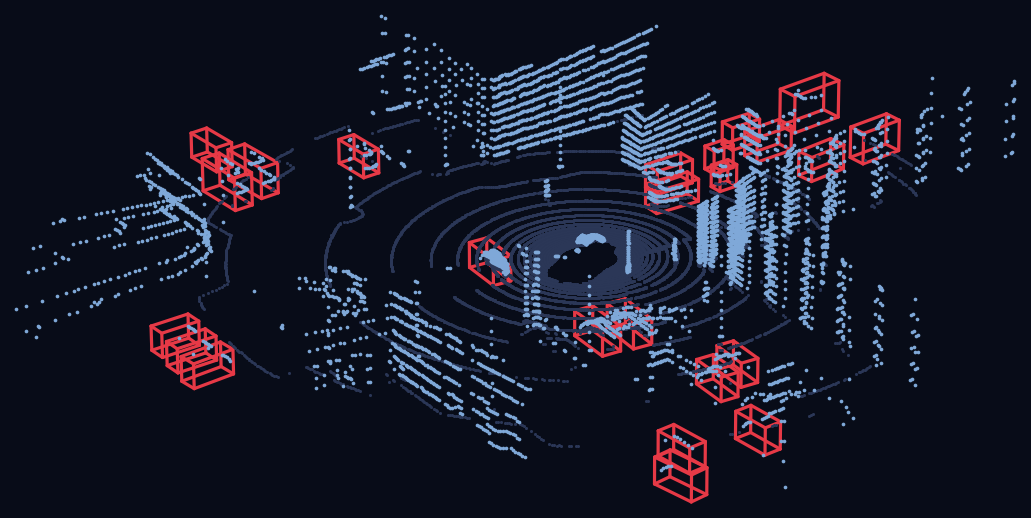
\includegraphics[height=2.30cm]{panels/detections.png}};
\draw[flow] (head-east) -- (det.west);
\node[mod, anchor=north, xshift=0.00cm, yshift=-0.10cm] at (45.424,-1.980,0) {\textbf{3-D}\\\textbf{boxes}};
% ====== auxiliary normal supervision - training only ======
\node[ellipse, draw=cLoss, fill=cLoss!8, line width=0.8pt, inner sep=2.5pt,
      text=cInk, align=center, font=\fontsize{18}{20}\selectfont]
      (ngfmloss) at (33.129,-4.000,0) {\textbf{NGFM loss}};
\draw[aux, draw=cLoss] (ngfm-south) -- (ngfmloss.north);
\draw[aux] (0.640,-1.150,0)
      -- (0.640,-4.000,0) -- (ngfmloss.west);
% ====== legend ======
\draw[flow] (35.879,-3.660,0) -- ++(0.85,0);
\draw[aux]  (35.879,-4.340,0) -- ++(0.85,0);
\node[tag, anchor=west, xshift=0.00cm, yshift=0.00cm] at (36.879,-3.660,0) {inference};
\node[tag, anchor=west, xshift=0.00cm, yshift=0.00cm] at (36.879,-4.340,0) {training only: offline surface normals};

\end{tikzpicture}
\end{document}
